\documentclass[12pt, a4paper, twoside, openany]{article}

\usepackage{sectsty}
\usepackage{multirow}
\usepackage{xcolor}
\usepackage{graphicx}

\begin{document}
    \allsectionsfont{\sffamily}

    \setlength{\parindent}{0 em}
    \setlength{\parskip}{1.5 ex plus 1 ex minus 1 ex}

    \section*{Brunn on Ubuntu}

    This Ubuntu installation comes with running versions of Bioclipse and
    Brunn. It has a user with sudo powers which you might want to change the
    password for. Here is a list of all passwords in the system: 

    \begin{center}
        \begin{tabular}{|c|l|l|}
        \hline
        Program & \multicolumn{2}{|c|}{User Credentials} \\
        \hline
        \multirow{2}{*}{Ubuntu} & username 
                                & \colorbox{yellow}{\texttt{brunn}} \\
                                & password 
                                & \colorbox{yellow}{\texttt{brunn}} \\
        \hline
        \multirow{2}{*}{MySQL}  & username 
                                & \colorbox{yellow}{\texttt{root}}  \\
                                & password 
                                & \colorbox{yellow}{\texttt{brunn}} \\
        \hline
        \end{tabular}
    \end{center}

    \section*{Brunn users}
    There are two Brunn users created in the Brunn database.

    \begin{center}
        \begin{tabular}{|c|l|l|}
            \hline
            User type & \multicolumn{2}{|c|}{User Credentials} \\
            \hline
            \multirow{2}{*}{Administrator} 
                           & username 
                           & \colorbox{yellow}{\texttt{admin}} \\
                           & password 
                           & \colorbox{yellow}{\texttt{admin}} \\
            \hline
            \multirow{2}{*}{Standard User} 
                           & username 
                           & \colorbox{yellow}{\texttt{user}}  \\
                           & password 
                           & \colorbox{yellow}{\texttt{user}}  \\
            \hline
        \end{tabular}
    \end{center}

    \newpage

    \section*{Getting started}
    Start Bioclipse from the desktop. Bioclipse should start with the Brunn
    view to the left. Double click the \texttt{Not Logged In} or right click
    and choose \texttt{Log In}.

    \begin{center}
        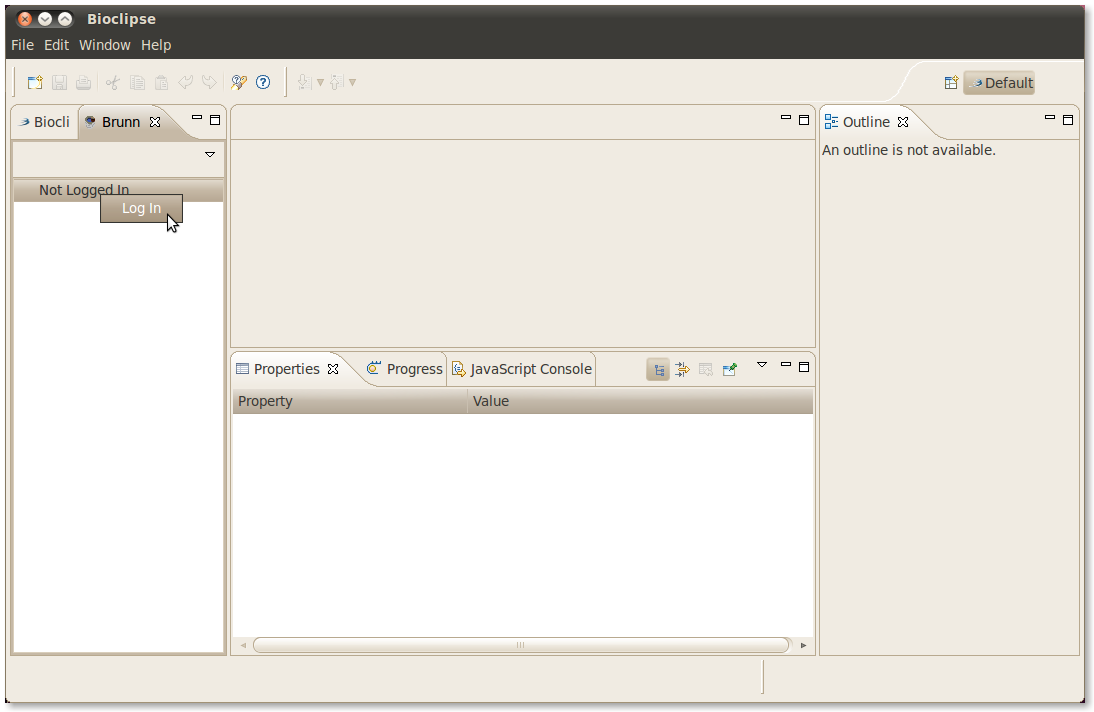
\includegraphics[scale=1.2]{images/1.png}
    \end{center}

    Log in as one of the Brunn users. For example, \texttt{admin} with password
    \texttt{admin}.

    \begin{center}
        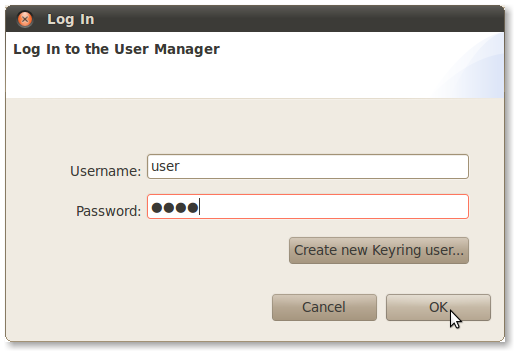
\includegraphics[scale=1.2]{images/2.png}
    \end{center}

    \newpage

    To access the Brunn help, click \texttt{Help} and \texttt{Help Contents}.

    \begin{center}
        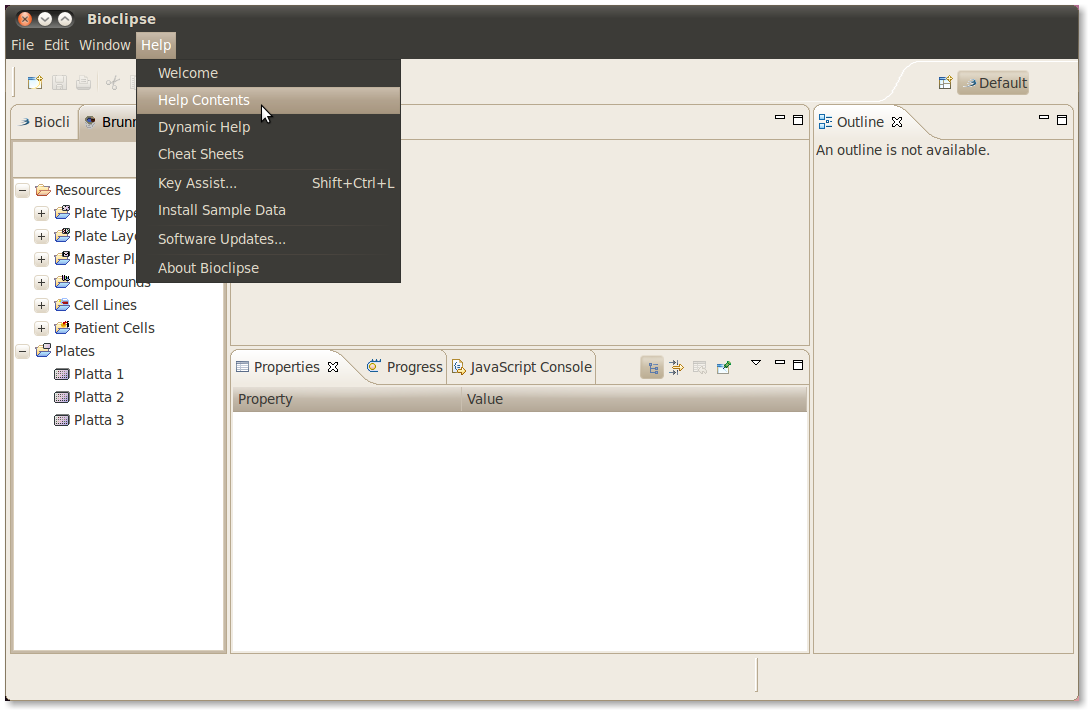
\includegraphics[scale=1.2]{images/5.png}
    \end{center}

    \begin{center}
        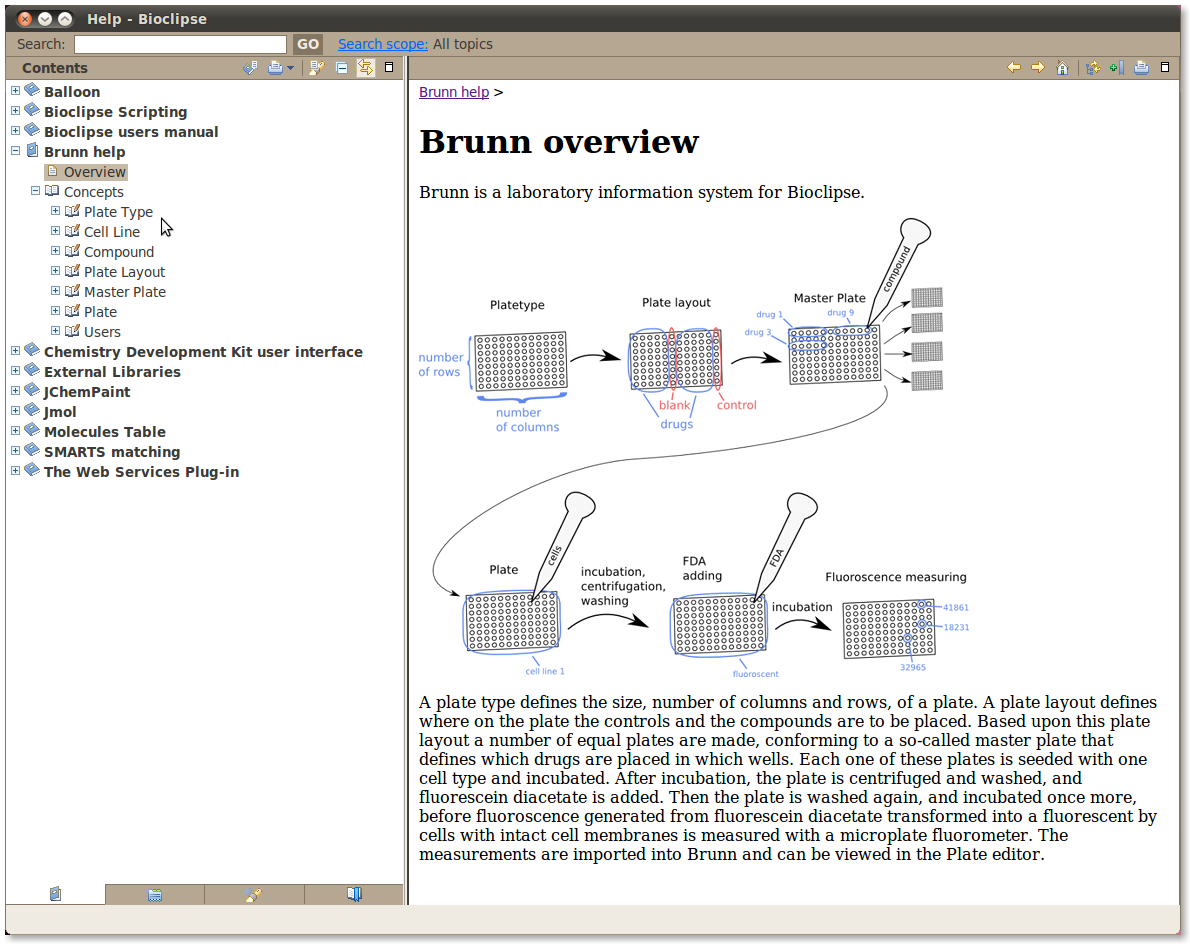
\includegraphics[scale=1.2]{images/6.png}
    \end{center}

    \newpage

    Cheat sheets are instructions for performing more specific tasks which can
    be shown inside the Bioclipse application. To open a cheat sheet, go to
    \texttt{Help} and \texttt{Cheat Sheets}, then select one of the Brunn cheat
    sheets.

    \begin{center}
        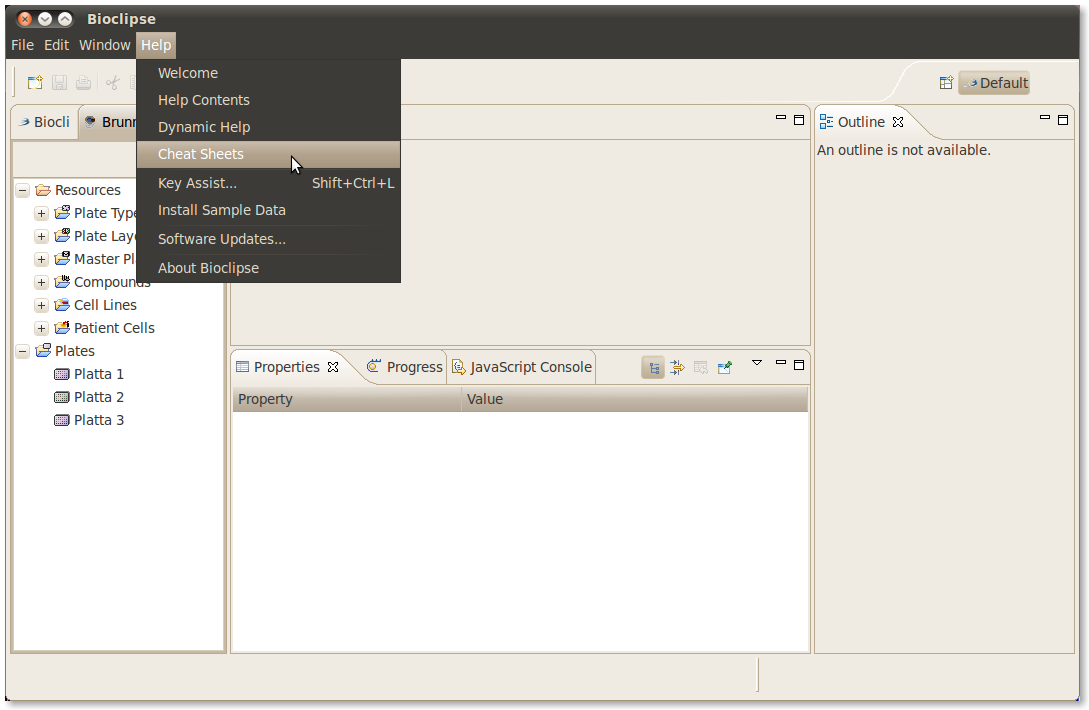
\includegraphics[height=35ex]{images/3.png}
        \hfill
        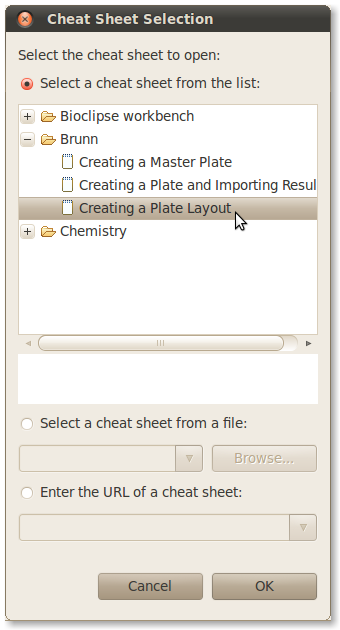
\includegraphics[height=35ex]{images/4.png}
    \end{center}

\end{document}
